% Created by tikzDevice version 0.12 on 2019-05-17 13:42:36
% !TEX encoding = UTF-8 Unicode
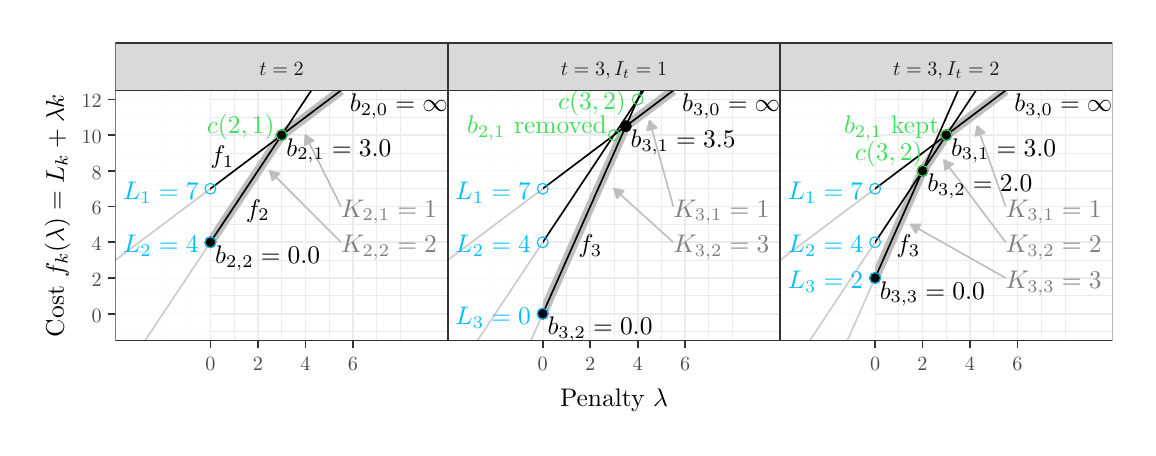
\begin{tikzpicture}[x=1pt,y=1pt]
\definecolor{fillColor}{RGB}{255,255,255}
\path[use as bounding box,fill=fillColor,fill opacity=0.00] (0,0) rectangle (397.48,144.54);
\begin{scope}
\path[clip] (  0.00,  0.00) rectangle (397.48,144.54);
\definecolor{drawColor}{RGB}{255,255,255}
\definecolor{fillColor}{RGB}{255,255,255}

\path[draw=drawColor,line width= 0.6pt,line join=round,line cap=round,fill=fillColor] ( -0.00,  0.00) rectangle (397.48,144.54);
\end{scope}
\begin{scope}
\path[clip] ( 31.72, 31.50) rectangle (151.81,121.85);
\definecolor{fillColor}{RGB}{255,255,255}

\path[fill=fillColor] ( 31.72, 31.50) rectangle (151.81,121.85);
\definecolor{drawColor}{gray}{0.92}

\path[draw=drawColor,line width= 0.3pt,line join=round] ( 31.72, 34.73) --
	(151.81, 34.73);

\path[draw=drawColor,line width= 0.3pt,line join=round] ( 31.72, 47.64) --
	(151.81, 47.64);

\path[draw=drawColor,line width= 0.3pt,line join=round] ( 31.72, 60.54) --
	(151.81, 60.54);

\path[draw=drawColor,line width= 0.3pt,line join=round] ( 31.72, 73.45) --
	(151.81, 73.45);

\path[draw=drawColor,line width= 0.3pt,line join=round] ( 31.72, 86.35) --
	(151.81, 86.35);

\path[draw=drawColor,line width= 0.3pt,line join=round] ( 31.72, 99.26) --
	(151.81, 99.26);

\path[draw=drawColor,line width= 0.3pt,line join=round] ( 31.72,112.17) --
	(151.81,112.17);

\path[draw=drawColor,line width= 0.3pt,line join=round] ( 48.88, 31.50) --
	( 48.88,121.85);

\path[draw=drawColor,line width= 0.3pt,line join=round] ( 57.46, 31.50) --
	( 57.46,121.85);

\path[draw=drawColor,line width= 0.3pt,line join=round] ( 74.61, 31.50) --
	( 74.61,121.85);

\path[draw=drawColor,line width= 0.3pt,line join=round] ( 91.77, 31.50) --
	( 91.77,121.85);

\path[draw=drawColor,line width= 0.3pt,line join=round] (108.92, 31.50) --
	(108.92,121.85);

\path[draw=drawColor,line width= 0.3pt,line join=round] (126.08, 31.50) --
	(126.08,121.85);

\path[draw=drawColor,line width= 0.3pt,line join=round] (134.66, 31.50) --
	(134.66,121.85);

\path[draw=drawColor,line width= 0.6pt,line join=round] ( 31.72, 41.18) --
	(151.81, 41.18);

\path[draw=drawColor,line width= 0.6pt,line join=round] ( 31.72, 54.09) --
	(151.81, 54.09);

\path[draw=drawColor,line width= 0.6pt,line join=round] ( 31.72, 66.99) --
	(151.81, 66.99);

\path[draw=drawColor,line width= 0.6pt,line join=round] ( 31.72, 79.90) --
	(151.81, 79.90);

\path[draw=drawColor,line width= 0.6pt,line join=round] ( 31.72, 92.81) --
	(151.81, 92.81);

\path[draw=drawColor,line width= 0.6pt,line join=round] ( 31.72,105.71) --
	(151.81,105.71);

\path[draw=drawColor,line width= 0.6pt,line join=round] ( 31.72,118.62) --
	(151.81,118.62);

\path[draw=drawColor,line width= 0.6pt,line join=round] ( 66.03, 31.50) --
	( 66.03,121.85);

\path[draw=drawColor,line width= 0.6pt,line join=round] ( 83.19, 31.50) --
	( 83.19,121.85);

\path[draw=drawColor,line width= 0.6pt,line join=round] (100.34, 31.50) --
	(100.34,121.85);

\path[draw=drawColor,line width= 0.6pt,line join=round] (117.50, 31.50) --
	(117.50,121.85);
\definecolor{drawColor}{RGB}{190,190,190}

\path[draw=drawColor,line width= 3.4pt,line join=round] ( 66.03, 66.99) --
	( 66.89, 68.29) --
	( 67.75, 69.58) --
	( 68.61, 70.87) --
	( 69.46, 72.16) --
	( 70.32, 73.45) --
	( 71.18, 74.74) --
	( 72.04, 76.03) --
	( 72.90, 77.32) --
	( 73.75, 78.61) --
	( 74.61, 79.90) --
	( 75.47, 81.19) --
	( 76.33, 82.48) --
	( 77.18, 83.77) --
	( 78.04, 85.06) --
	( 78.90, 86.35) --
	( 79.76, 87.64) --
	( 80.62, 88.94) --
	( 81.47, 90.23) --
	( 82.33, 91.52) --
	( 83.19, 92.81) --
	( 84.05, 94.10) --
	( 84.90, 95.39) --
	( 85.76, 96.68) --
	( 86.62, 97.97) --
	( 87.48, 99.26) --
	( 88.34,100.55) --
	( 89.19,101.84) --
	( 90.05,103.13) --
	( 90.91,104.42) --
	( 91.77,105.71) --
	( 92.62,106.36) --
	( 93.48,107.00) --
	( 94.34,107.65) --
	( 95.20,108.30) --
	( 96.06,108.94) --
	( 96.91,109.59) --
	( 97.77,110.23) --
	( 98.63,110.88) --
	( 99.49,111.52) --
	(100.34,112.17) --
	(101.20,112.81) --
	(102.06,113.46) --
	(102.92,114.10) --
	(103.78,114.75) --
	(104.63,115.39) --
	(105.49,116.04) --
	(106.35,116.68) --
	(107.21,117.33) --
	(108.06,117.97) --
	(108.92,118.62) --
	(109.78,119.27) --
	(110.64,119.91) --
	(111.50,120.56) --
	(112.35,121.20) --
	(113.21,121.85);

\path[draw=drawColor,line width= 0.6pt,line join=round] (113.21, 79.90) -- (100.34,105.71);
\definecolor{fillColor}{RGB}{190,190,190}

\path[draw=drawColor,line width= 0.6pt,line join=round,fill=fillColor] (103.36,103.72) --
	(100.34,105.71) --
	(100.12,102.11) --
	cycle;

\path[draw=drawColor,line width= 0.6pt,line join=round] (113.21, 66.99) -- ( 87.48, 92.81);

\path[draw=drawColor,line width= 0.6pt,line join=round,fill=fillColor] ( 90.97, 91.87) --
	( 87.48, 92.81) --
	( 88.41, 89.32) --
	cycle;
\definecolor{drawColor}{RGB}{0,0,0}

\node[text=drawColor,anchor=base west,inner sep=0pt, outer sep=0pt, scale=  0.92] at ( 67.75, 59.39) {$b_{2,2}=0.0$};

\node[text=drawColor,anchor=base west,inner sep=0pt, outer sep=0pt, scale=  0.92] at ( 93.48, 98.11) {$b_{2,1}=3.0$};

\path[draw=drawColor,line width= 0.6pt,line join=round] ( 31.72, 60.54) -- (143.38,144.54);

\path[draw=drawColor,line width= 0.6pt,line join=round] ( 31.72, 15.37) -- (117.57,144.54);
\definecolor{fillColor}{RGB}{255,255,255}

\path[fill=fillColor,fill opacity=0.80] ( 31.72, 31.50) rectangle ( 66.03,121.85);
\definecolor{drawColor}{gray}{0.50}

\node[text=drawColor,anchor=base west,inner sep=0pt, outer sep=0pt, scale=  0.92] at (113.21, 76.10) {$K_{2,1}=1$};

\node[text=drawColor,anchor=base west,inner sep=0pt, outer sep=0pt, scale=  0.92] at (113.21, 63.19) {$K_{2,2}=2$};
\definecolor{drawColor}{RGB}{0,0,0}
\definecolor{fillColor}{RGB}{0,0,0}

\path[draw=drawColor,line width= 0.4pt,line join=round,line cap=round,fill=fillColor] ( 66.03, 66.99) circle (  1.96);

\path[draw=drawColor,line width= 0.4pt,line join=round,line cap=round,fill=fillColor] ( 91.77,105.71) circle (  1.96);
\definecolor{drawColor}{RGB}{65,221,93}

\path[draw=drawColor,line width= 0.4pt,line join=round,line cap=round] ( 91.77,105.71) circle (  1.96);

\node[text=drawColor,anchor=base east,inner sep=0pt, outer sep=0pt, scale=  0.92] at ( 89.19,106.36) {$c(2, 1)$};
\definecolor{drawColor}{RGB}{0,0,0}

\node[text=drawColor,anchor=base,inner sep=0pt, outer sep=0pt, scale=  0.92] at ( 70.32, 95.46) {$f_1$};

\node[text=drawColor,anchor=base,inner sep=0pt, outer sep=0pt, scale=  0.92] at ( 83.19, 76.10) {$f_2$};

\node[text=drawColor,anchor=base east,inner sep=0pt, outer sep=0pt, scale=  0.92] at (151.81,114.24) {$b_{2,0}=\infty$};
\definecolor{drawColor}{RGB}{0,191,255}

\node[text=drawColor,anchor=base east,inner sep=0pt, outer sep=0pt, scale=  0.92] at ( 61.75, 82.55) {$L_1=7$};

\node[text=drawColor,anchor=base east,inner sep=0pt, outer sep=0pt, scale=  0.92] at ( 61.75, 63.19) {$L_2=4$};

\path[draw=drawColor,line width= 0.4pt,line join=round,line cap=round] ( 66.03, 86.35) circle (  1.96);

\path[draw=drawColor,line width= 0.4pt,line join=round,line cap=round] ( 66.03, 66.99) circle (  1.96);
\definecolor{drawColor}{gray}{0.20}

\path[draw=drawColor,line width= 0.6pt,line join=round,line cap=round] ( 31.72, 31.50) rectangle (151.81,121.85);
\end{scope}
\begin{scope}
\path[clip] (151.81, 31.50) rectangle (271.90,121.85);
\definecolor{fillColor}{RGB}{255,255,255}

\path[fill=fillColor] (151.81, 31.50) rectangle (271.90,121.85);
\definecolor{drawColor}{gray}{0.92}

\path[draw=drawColor,line width= 0.3pt,line join=round] (151.81, 34.73) --
	(271.90, 34.73);

\path[draw=drawColor,line width= 0.3pt,line join=round] (151.81, 47.64) --
	(271.90, 47.64);

\path[draw=drawColor,line width= 0.3pt,line join=round] (151.81, 60.54) --
	(271.90, 60.54);

\path[draw=drawColor,line width= 0.3pt,line join=round] (151.81, 73.45) --
	(271.90, 73.45);

\path[draw=drawColor,line width= 0.3pt,line join=round] (151.81, 86.35) --
	(271.90, 86.35);

\path[draw=drawColor,line width= 0.3pt,line join=round] (151.81, 99.26) --
	(271.90, 99.26);

\path[draw=drawColor,line width= 0.3pt,line join=round] (151.81,112.17) --
	(271.90,112.17);

\path[draw=drawColor,line width= 0.3pt,line join=round] (168.97, 31.50) --
	(168.97,121.85);

\path[draw=drawColor,line width= 0.3pt,line join=round] (177.54, 31.50) --
	(177.54,121.85);

\path[draw=drawColor,line width= 0.3pt,line join=round] (194.70, 31.50) --
	(194.70,121.85);

\path[draw=drawColor,line width= 0.3pt,line join=round] (211.85, 31.50) --
	(211.85,121.85);

\path[draw=drawColor,line width= 0.3pt,line join=round] (229.01, 31.50) --
	(229.01,121.85);

\path[draw=drawColor,line width= 0.3pt,line join=round] (246.16, 31.50) --
	(246.16,121.85);

\path[draw=drawColor,line width= 0.3pt,line join=round] (254.74, 31.50) --
	(254.74,121.85);

\path[draw=drawColor,line width= 0.6pt,line join=round] (151.81, 41.18) --
	(271.90, 41.18);

\path[draw=drawColor,line width= 0.6pt,line join=round] (151.81, 54.09) --
	(271.90, 54.09);

\path[draw=drawColor,line width= 0.6pt,line join=round] (151.81, 66.99) --
	(271.90, 66.99);

\path[draw=drawColor,line width= 0.6pt,line join=round] (151.81, 79.90) --
	(271.90, 79.90);

\path[draw=drawColor,line width= 0.6pt,line join=round] (151.81, 92.81) --
	(271.90, 92.81);

\path[draw=drawColor,line width= 0.6pt,line join=round] (151.81,105.71) --
	(271.90,105.71);

\path[draw=drawColor,line width= 0.6pt,line join=round] (151.81,118.62) --
	(271.90,118.62);

\path[draw=drawColor,line width= 0.6pt,line join=round] (186.12, 31.50) --
	(186.12,121.85);

\path[draw=drawColor,line width= 0.6pt,line join=round] (203.28, 31.50) --
	(203.28,121.85);

\path[draw=drawColor,line width= 0.6pt,line join=round] (220.43, 31.50) --
	(220.43,121.85);

\path[draw=drawColor,line width= 0.6pt,line join=round] (237.59, 31.50) --
	(237.59,121.85);
\definecolor{drawColor}{RGB}{190,190,190}

\path[draw=drawColor,line width= 3.4pt,line join=round] (186.12, 41.18) --
	(186.98, 43.12) --
	(187.84, 45.05) --
	(188.69, 46.99) --
	(189.55, 48.93) --
	(190.41, 50.86) --
	(191.27, 52.80) --
	(192.13, 54.73) --
	(192.98, 56.67) --
	(193.84, 58.61) --
	(194.70, 60.54) --
	(195.56, 62.48) --
	(196.41, 64.41) --
	(197.27, 66.35) --
	(198.13, 68.29) --
	(198.99, 70.22) --
	(199.85, 72.16) --
	(200.70, 74.09) --
	(201.56, 76.03) --
	(202.42, 77.97) --
	(203.28, 79.90) --
	(204.13, 81.84) --
	(204.99, 83.77) --
	(205.85, 85.71) --
	(206.71, 87.64) --
	(207.57, 89.58) --
	(208.42, 91.52) --
	(209.28, 93.45) --
	(210.14, 95.39) --
	(211.00, 97.32) --
	(211.85, 99.26) --
	(212.71,101.20) --
	(213.57,103.13) --
	(214.43,105.07) --
	(215.29,107.00) --
	(216.14,108.94) --
	(217.00,109.59) --
	(217.86,110.23) --
	(218.72,110.88) --
	(219.57,111.52) --
	(220.43,112.17) --
	(221.29,112.81) --
	(222.15,113.46) --
	(223.01,114.10) --
	(223.86,114.75) --
	(224.72,115.39) --
	(225.58,116.04) --
	(226.44,116.68) --
	(227.29,117.33) --
	(228.15,117.97) --
	(229.01,118.62) --
	(229.87,119.27) --
	(230.72,119.91) --
	(231.58,120.56) --
	(232.44,121.20) --
	(233.30,121.85);

\path[draw=drawColor,line width= 0.6pt,line join=round] (233.30, 79.90) -- (224.72,110.88);
\definecolor{fillColor}{RGB}{190,190,190}

\path[draw=drawColor,line width= 0.6pt,line join=round,fill=fillColor] (227.30,108.34) --
	(224.72,110.88) --
	(223.81,107.38) --
	cycle;

\path[draw=drawColor,line width= 0.6pt,line join=round] (233.30, 66.99) -- (211.85, 86.35);

\path[draw=drawColor,line width= 0.6pt,line join=round,fill=fillColor] (215.39, 85.60) --
	(211.85, 86.35) --
	(212.97, 82.92) --
	cycle;
\definecolor{drawColor}{RGB}{0,0,0}

\node[text=drawColor,anchor=base west,inner sep=0pt, outer sep=0pt, scale=  0.92] at (187.84, 33.58) {$b_{3,2}=0.0$};

\node[text=drawColor,anchor=base west,inner sep=0pt, outer sep=0pt, scale=  0.92] at (217.86,101.34) {$b_{3,1}=3.5$};

\path[draw=drawColor,line width= 0.6pt,line join=round] (151.81, 60.54) -- (263.46,144.54);

\path[draw=drawColor,line width= 0.6pt,line join=round] (151.81, 15.37) -- (237.66,144.54);

\path[draw=drawColor,line width= 0.6pt,line join=round] (167.87,  0.00) -- (231.92,144.54);
\definecolor{fillColor}{RGB}{255,255,255}

\path[fill=fillColor,fill opacity=0.80] (151.81, 31.50) rectangle (186.12,121.85);
\definecolor{drawColor}{gray}{0.50}

\node[text=drawColor,anchor=base west,inner sep=0pt, outer sep=0pt, scale=  0.92] at (233.30, 76.10) {$K_{3,1}=1$};

\node[text=drawColor,anchor=base west,inner sep=0pt, outer sep=0pt, scale=  0.92] at (233.30, 63.19) {$K_{3,2}=3$};
\definecolor{drawColor}{RGB}{0,0,0}
\definecolor{fillColor}{RGB}{0,0,0}

\path[draw=drawColor,line width= 0.4pt,line join=round,line cap=round,fill=fillColor] (186.12, 41.18) circle (  1.96);

\path[draw=drawColor,line width= 0.4pt,line join=round,line cap=round,fill=fillColor] (216.14,108.94) circle (  1.96);
\definecolor{drawColor}{RGB}{65,221,93}

\path[draw=drawColor,line width= 0.4pt,line join=round,line cap=round] (211.85,105.71) circle (  1.96);

\path[draw=drawColor,line width= 0.4pt,line join=round,line cap=round] (220.43,118.62) circle (  1.96);

\node[text=drawColor,anchor=base east,inner sep=0pt, outer sep=0pt, scale=  0.92] at (216.14,114.82) {$c(3, 2)$};

\node[text=drawColor,anchor=base east,inner sep=0pt, outer sep=0pt, scale=  0.92] at (209.28,106.36) {$b_{2,1}$ removed};
\definecolor{drawColor}{RGB}{0,0,0}

\node[text=drawColor,anchor=base,inner sep=0pt, outer sep=0pt, scale=  0.92] at (203.28, 63.19) {$f_3$};

\node[text=drawColor,anchor=base east,inner sep=0pt, outer sep=0pt, scale=  0.92] at (271.90,114.24) {$b_{3,0}=\infty$};
\definecolor{drawColor}{RGB}{0,191,255}

\node[text=drawColor,anchor=base east,inner sep=0pt, outer sep=0pt, scale=  0.92] at (181.83, 82.55) {$L_1=7$};

\node[text=drawColor,anchor=base east,inner sep=0pt, outer sep=0pt, scale=  0.92] at (181.83, 63.19) {$L_2=4$};

\node[text=drawColor,anchor=base east,inner sep=0pt, outer sep=0pt, scale=  0.92] at (181.83, 37.38) {$L_3=0$};

\path[draw=drawColor,line width= 0.4pt,line join=round,line cap=round] (186.12, 86.35) circle (  1.96);

\path[draw=drawColor,line width= 0.4pt,line join=round,line cap=round] (186.12, 66.99) circle (  1.96);

\path[draw=drawColor,line width= 0.4pt,line join=round,line cap=round] (186.12, 41.18) circle (  1.96);
\definecolor{drawColor}{gray}{0.20}

\path[draw=drawColor,line width= 0.6pt,line join=round,line cap=round] (151.81, 31.50) rectangle (271.90,121.85);
\end{scope}
\begin{scope}
\path[clip] (271.90, 31.50) rectangle (391.98,121.85);
\definecolor{fillColor}{RGB}{255,255,255}

\path[fill=fillColor] (271.90, 31.50) rectangle (391.98,121.85);
\definecolor{drawColor}{gray}{0.92}

\path[draw=drawColor,line width= 0.3pt,line join=round] (271.90, 34.73) --
	(391.98, 34.73);

\path[draw=drawColor,line width= 0.3pt,line join=round] (271.90, 47.64) --
	(391.98, 47.64);

\path[draw=drawColor,line width= 0.3pt,line join=round] (271.90, 60.54) --
	(391.98, 60.54);

\path[draw=drawColor,line width= 0.3pt,line join=round] (271.90, 73.45) --
	(391.98, 73.45);

\path[draw=drawColor,line width= 0.3pt,line join=round] (271.90, 86.35) --
	(391.98, 86.35);

\path[draw=drawColor,line width= 0.3pt,line join=round] (271.90, 99.26) --
	(391.98, 99.26);

\path[draw=drawColor,line width= 0.3pt,line join=round] (271.90,112.17) --
	(391.98,112.17);

\path[draw=drawColor,line width= 0.3pt,line join=round] (289.05, 31.50) --
	(289.05,121.85);

\path[draw=drawColor,line width= 0.3pt,line join=round] (297.63, 31.50) --
	(297.63,121.85);

\path[draw=drawColor,line width= 0.3pt,line join=round] (314.79, 31.50) --
	(314.79,121.85);

\path[draw=drawColor,line width= 0.3pt,line join=round] (331.94, 31.50) --
	(331.94,121.85);

\path[draw=drawColor,line width= 0.3pt,line join=round] (349.10, 31.50) --
	(349.10,121.85);

\path[draw=drawColor,line width= 0.3pt,line join=round] (366.25, 31.50) --
	(366.25,121.85);

\path[draw=drawColor,line width= 0.3pt,line join=round] (374.83, 31.50) --
	(374.83,121.85);

\path[draw=drawColor,line width= 0.6pt,line join=round] (271.90, 41.18) --
	(391.98, 41.18);

\path[draw=drawColor,line width= 0.6pt,line join=round] (271.90, 54.09) --
	(391.98, 54.09);

\path[draw=drawColor,line width= 0.6pt,line join=round] (271.90, 66.99) --
	(391.98, 66.99);

\path[draw=drawColor,line width= 0.6pt,line join=round] (271.90, 79.90) --
	(391.98, 79.90);

\path[draw=drawColor,line width= 0.6pt,line join=round] (271.90, 92.81) --
	(391.98, 92.81);

\path[draw=drawColor,line width= 0.6pt,line join=round] (271.90,105.71) --
	(391.98,105.71);

\path[draw=drawColor,line width= 0.6pt,line join=round] (271.90,118.62) --
	(391.98,118.62);

\path[draw=drawColor,line width= 0.6pt,line join=round] (306.21, 31.50) --
	(306.21,121.85);

\path[draw=drawColor,line width= 0.6pt,line join=round] (323.36, 31.50) --
	(323.36,121.85);

\path[draw=drawColor,line width= 0.6pt,line join=round] (340.52, 31.50) --
	(340.52,121.85);

\path[draw=drawColor,line width= 0.6pt,line join=round] (357.67, 31.50) --
	(357.67,121.85);
\definecolor{drawColor}{RGB}{190,190,190}

\path[draw=drawColor,line width= 3.4pt,line join=round] (306.21, 54.09) --
	(307.07, 56.02) --
	(307.92, 57.96) --
	(308.78, 59.90) --
	(309.64, 61.83) --
	(310.50, 63.77) --
	(311.35, 65.70) --
	(312.21, 67.64) --
	(313.07, 69.58) --
	(313.93, 71.51) --
	(314.79, 73.45) --
	(315.64, 75.38) --
	(316.50, 77.32) --
	(317.36, 79.26) --
	(318.22, 81.19) --
	(319.07, 83.13) --
	(319.93, 85.06) --
	(320.79, 87.00) --
	(321.65, 88.94) --
	(322.51, 90.87) --
	(323.36, 92.81) --
	(324.22, 94.10) --
	(325.08, 95.39) --
	(325.94, 96.68) --
	(326.79, 97.97) --
	(327.65, 99.26) --
	(328.51,100.55) --
	(329.37,101.84) --
	(330.23,103.13) --
	(331.08,104.42) --
	(331.94,105.71) --
	(332.80,106.36) --
	(333.66,107.00) --
	(334.51,107.65) --
	(335.37,108.30) --
	(336.23,108.94) --
	(337.09,109.59) --
	(337.95,110.23) --
	(338.80,110.88) --
	(339.66,111.52) --
	(340.52,112.17) --
	(341.38,112.81) --
	(342.23,113.46) --
	(343.09,114.10) --
	(343.95,114.75) --
	(344.81,115.39) --
	(345.67,116.04) --
	(346.52,116.68) --
	(347.38,117.33) --
	(348.24,117.97) --
	(349.10,118.62) --
	(349.95,119.27) --
	(350.81,119.91) --
	(351.67,120.56) --
	(352.53,121.20) --
	(353.39,121.85);

\path[draw=drawColor,line width= 0.6pt,line join=round] (353.39, 79.90) -- (343.09,108.94);
\definecolor{fillColor}{RGB}{190,190,190}

\path[draw=drawColor,line width= 0.6pt,line join=round,fill=fillColor] (345.84,106.59) --
	(343.09,108.94) --
	(342.43,105.39) --
	cycle;

\path[draw=drawColor,line width= 0.6pt,line join=round] (353.39, 66.99) -- (331.08, 96.68);

\path[draw=drawColor,line width= 0.6pt,line join=round,fill=fillColor] (334.41, 95.26) --
	(331.08, 96.68) --
	(331.52, 93.09) --
	cycle;

\path[draw=drawColor,line width= 0.6pt,line join=round] (353.39, 54.09) -- (319.07, 73.45);

\path[draw=drawColor,line width= 0.6pt,line join=round,fill=fillColor] (322.69, 73.48) --
	(319.07, 73.45) --
	(320.91, 70.34) --
	cycle;
\definecolor{drawColor}{RGB}{0,0,0}

\node[text=drawColor,anchor=base west,inner sep=0pt, outer sep=0pt, scale=  0.92] at (307.92, 46.48) {$b_{3,3}=0.0$};

\node[text=drawColor,anchor=base west,inner sep=0pt, outer sep=0pt, scale=  0.92] at (325.08, 85.20) {$b_{3,2}=2.0$};

\node[text=drawColor,anchor=base west,inner sep=0pt, outer sep=0pt, scale=  0.92] at (333.66, 98.11) {$b_{3,1}=3.0$};

\path[draw=drawColor,line width= 0.6pt,line join=round] (271.90, 60.54) -- (383.55,144.54);

\path[draw=drawColor,line width= 0.6pt,line join=round] (271.90, 15.37) -- (357.75,144.54);

\path[draw=drawColor,line width= 0.6pt,line join=round] (282.24,  0.00) -- (346.28,144.54);
\definecolor{fillColor}{RGB}{255,255,255}

\path[fill=fillColor,fill opacity=0.80] (271.90, 31.50) rectangle (306.21,121.85);
\definecolor{drawColor}{gray}{0.50}

\node[text=drawColor,anchor=base west,inner sep=0pt, outer sep=0pt, scale=  0.92] at (353.39, 76.10) {$K_{3,1}=1$};

\node[text=drawColor,anchor=base west,inner sep=0pt, outer sep=0pt, scale=  0.92] at (353.39, 63.19) {$K_{3,2}=2$};

\node[text=drawColor,anchor=base west,inner sep=0pt, outer sep=0pt, scale=  0.92] at (353.39, 50.29) {$K_{3,3}=3$};
\definecolor{drawColor}{RGB}{0,0,0}
\definecolor{fillColor}{RGB}{0,0,0}

\path[draw=drawColor,line width= 0.4pt,line join=round,line cap=round,fill=fillColor] (306.21, 54.09) circle (  1.96);

\path[draw=drawColor,line width= 0.4pt,line join=round,line cap=round,fill=fillColor] (323.36, 92.81) circle (  1.96);

\path[draw=drawColor,line width= 0.4pt,line join=round,line cap=round,fill=fillColor] (331.94,105.71) circle (  1.96);
\definecolor{drawColor}{RGB}{65,221,93}

\path[draw=drawColor,line width= 0.4pt,line join=round,line cap=round] (331.94,105.71) circle (  1.96);

\path[draw=drawColor,line width= 0.4pt,line join=round,line cap=round] (323.36, 92.81) circle (  1.96);

\node[text=drawColor,anchor=base east,inner sep=0pt, outer sep=0pt, scale=  0.92] at (323.36, 96.61) {$c(3, 2)$};

\node[text=drawColor,anchor=base east,inner sep=0pt, outer sep=0pt, scale=  0.92] at (329.37,106.36) {$b_{2,1}$ kept};
\definecolor{drawColor}{RGB}{0,0,0}

\node[text=drawColor,anchor=base,inner sep=0pt, outer sep=0pt, scale=  0.92] at (318.22, 63.19) {$f_3$};

\node[text=drawColor,anchor=base east,inner sep=0pt, outer sep=0pt, scale=  0.92] at (391.98,114.24) {$b_{3,0}=\infty$};
\definecolor{drawColor}{RGB}{0,191,255}

\node[text=drawColor,anchor=base east,inner sep=0pt, outer sep=0pt, scale=  0.92] at (301.92, 82.55) {$L_1=7$};

\node[text=drawColor,anchor=base east,inner sep=0pt, outer sep=0pt, scale=  0.92] at (301.92, 63.19) {$L_2=4$};

\node[text=drawColor,anchor=base east,inner sep=0pt, outer sep=0pt, scale=  0.92] at (301.92, 50.29) {$L_3=2$};

\path[draw=drawColor,line width= 0.4pt,line join=round,line cap=round] (306.21, 86.35) circle (  1.96);

\path[draw=drawColor,line width= 0.4pt,line join=round,line cap=round] (306.21, 66.99) circle (  1.96);

\path[draw=drawColor,line width= 0.4pt,line join=round,line cap=round] (306.21, 54.09) circle (  1.96);
\definecolor{drawColor}{gray}{0.20}

\path[draw=drawColor,line width= 0.6pt,line join=round,line cap=round] (271.90, 31.50) rectangle (391.98,121.85);
\end{scope}
\begin{scope}
\path[clip] ( 31.72,121.85) rectangle (151.81,139.04);
\definecolor{drawColor}{gray}{0.20}
\definecolor{fillColor}{gray}{0.85}

\path[draw=drawColor,line width= 0.6pt,line join=round,line cap=round,fill=fillColor] ( 31.72,121.85) rectangle (151.81,139.04);
\definecolor{drawColor}{gray}{0.10}

\node[text=drawColor,anchor=base,inner sep=0pt, outer sep=0pt, scale=  0.73] at ( 91.77,127.41) {$t=2$};
\end{scope}
\begin{scope}
\path[clip] (151.81,121.85) rectangle (271.90,139.04);
\definecolor{drawColor}{gray}{0.20}
\definecolor{fillColor}{gray}{0.85}

\path[draw=drawColor,line width= 0.6pt,line join=round,line cap=round,fill=fillColor] (151.81,121.85) rectangle (271.90,139.04);
\definecolor{drawColor}{gray}{0.10}

\node[text=drawColor,anchor=base,inner sep=0pt, outer sep=0pt, scale=  0.73] at (211.85,127.41) {$t=3, I_t=1$};
\end{scope}
\begin{scope}
\path[clip] (271.90,121.85) rectangle (391.98,139.04);
\definecolor{drawColor}{gray}{0.20}
\definecolor{fillColor}{gray}{0.85}

\path[draw=drawColor,line width= 0.6pt,line join=round,line cap=round,fill=fillColor] (271.90,121.85) rectangle (391.98,139.04);
\definecolor{drawColor}{gray}{0.10}

\node[text=drawColor,anchor=base,inner sep=0pt, outer sep=0pt, scale=  0.73] at (331.94,127.41) {$t=3, I_t=2$};
\end{scope}
\begin{scope}
\path[clip] (  0.00,  0.00) rectangle (397.48,144.54);
\definecolor{drawColor}{gray}{0.20}

\path[draw=drawColor,line width= 0.6pt,line join=round] ( 66.03, 28.75) --
	( 66.03, 31.50);

\path[draw=drawColor,line width= 0.6pt,line join=round] ( 83.19, 28.75) --
	( 83.19, 31.50);

\path[draw=drawColor,line width= 0.6pt,line join=round] (100.34, 28.75) --
	(100.34, 31.50);

\path[draw=drawColor,line width= 0.6pt,line join=round] (117.50, 28.75) --
	(117.50, 31.50);
\end{scope}
\begin{scope}
\path[clip] (  0.00,  0.00) rectangle (397.48,144.54);
\definecolor{drawColor}{gray}{0.30}

\node[text=drawColor,anchor=base,inner sep=0pt, outer sep=0pt, scale=  0.73] at ( 66.03, 20.49) {0};

\node[text=drawColor,anchor=base,inner sep=0pt, outer sep=0pt, scale=  0.73] at ( 83.19, 20.49) {2};

\node[text=drawColor,anchor=base,inner sep=0pt, outer sep=0pt, scale=  0.73] at (100.34, 20.49) {4};

\node[text=drawColor,anchor=base,inner sep=0pt, outer sep=0pt, scale=  0.73] at (117.50, 20.49) {6};
\end{scope}
\begin{scope}
\path[clip] (  0.00,  0.00) rectangle (397.48,144.54);
\definecolor{drawColor}{gray}{0.20}

\path[draw=drawColor,line width= 0.6pt,line join=round] (186.12, 28.75) --
	(186.12, 31.50);

\path[draw=drawColor,line width= 0.6pt,line join=round] (203.28, 28.75) --
	(203.28, 31.50);

\path[draw=drawColor,line width= 0.6pt,line join=round] (220.43, 28.75) --
	(220.43, 31.50);

\path[draw=drawColor,line width= 0.6pt,line join=round] (237.59, 28.75) --
	(237.59, 31.50);
\end{scope}
\begin{scope}
\path[clip] (  0.00,  0.00) rectangle (397.48,144.54);
\definecolor{drawColor}{gray}{0.30}

\node[text=drawColor,anchor=base,inner sep=0pt, outer sep=0pt, scale=  0.73] at (186.12, 20.49) {0};

\node[text=drawColor,anchor=base,inner sep=0pt, outer sep=0pt, scale=  0.73] at (203.28, 20.49) {2};

\node[text=drawColor,anchor=base,inner sep=0pt, outer sep=0pt, scale=  0.73] at (220.43, 20.49) {4};

\node[text=drawColor,anchor=base,inner sep=0pt, outer sep=0pt, scale=  0.73] at (237.59, 20.49) {6};
\end{scope}
\begin{scope}
\path[clip] (  0.00,  0.00) rectangle (397.48,144.54);
\definecolor{drawColor}{gray}{0.20}

\path[draw=drawColor,line width= 0.6pt,line join=round] (306.21, 28.75) --
	(306.21, 31.50);

\path[draw=drawColor,line width= 0.6pt,line join=round] (323.36, 28.75) --
	(323.36, 31.50);

\path[draw=drawColor,line width= 0.6pt,line join=round] (340.52, 28.75) --
	(340.52, 31.50);

\path[draw=drawColor,line width= 0.6pt,line join=round] (357.67, 28.75) --
	(357.67, 31.50);
\end{scope}
\begin{scope}
\path[clip] (  0.00,  0.00) rectangle (397.48,144.54);
\definecolor{drawColor}{gray}{0.30}

\node[text=drawColor,anchor=base,inner sep=0pt, outer sep=0pt, scale=  0.73] at (306.21, 20.49) {0};

\node[text=drawColor,anchor=base,inner sep=0pt, outer sep=0pt, scale=  0.73] at (323.36, 20.49) {2};

\node[text=drawColor,anchor=base,inner sep=0pt, outer sep=0pt, scale=  0.73] at (340.52, 20.49) {4};

\node[text=drawColor,anchor=base,inner sep=0pt, outer sep=0pt, scale=  0.73] at (357.67, 20.49) {6};
\end{scope}
\begin{scope}
\path[clip] (  0.00,  0.00) rectangle (397.48,144.54);
\definecolor{drawColor}{gray}{0.30}

\node[text=drawColor,anchor=base east,inner sep=0pt, outer sep=0pt, scale=  0.73] at ( 26.77, 38.15) {0};

\node[text=drawColor,anchor=base east,inner sep=0pt, outer sep=0pt, scale=  0.73] at ( 26.77, 51.06) {2};

\node[text=drawColor,anchor=base east,inner sep=0pt, outer sep=0pt, scale=  0.73] at ( 26.77, 63.96) {4};

\node[text=drawColor,anchor=base east,inner sep=0pt, outer sep=0pt, scale=  0.73] at ( 26.77, 76.87) {6};

\node[text=drawColor,anchor=base east,inner sep=0pt, outer sep=0pt, scale=  0.73] at ( 26.77, 89.78) {8};

\node[text=drawColor,anchor=base east,inner sep=0pt, outer sep=0pt, scale=  0.73] at ( 26.77,102.68) {10};

\node[text=drawColor,anchor=base east,inner sep=0pt, outer sep=0pt, scale=  0.73] at ( 26.77,115.59) {12};
\end{scope}
\begin{scope}
\path[clip] (  0.00,  0.00) rectangle (397.48,144.54);
\definecolor{drawColor}{gray}{0.20}

\path[draw=drawColor,line width= 0.6pt,line join=round] ( 28.97, 41.18) --
	( 31.72, 41.18);

\path[draw=drawColor,line width= 0.6pt,line join=round] ( 28.97, 54.09) --
	( 31.72, 54.09);

\path[draw=drawColor,line width= 0.6pt,line join=round] ( 28.97, 66.99) --
	( 31.72, 66.99);

\path[draw=drawColor,line width= 0.6pt,line join=round] ( 28.97, 79.90) --
	( 31.72, 79.90);

\path[draw=drawColor,line width= 0.6pt,line join=round] ( 28.97, 92.81) --
	( 31.72, 92.81);

\path[draw=drawColor,line width= 0.6pt,line join=round] ( 28.97,105.71) --
	( 31.72,105.71);

\path[draw=drawColor,line width= 0.6pt,line join=round] ( 28.97,118.62) --
	( 31.72,118.62);
\end{scope}
\begin{scope}
\path[clip] (  0.00,  0.00) rectangle (397.48,144.54);
\definecolor{drawColor}{RGB}{0,0,0}

\node[text=drawColor,anchor=base,inner sep=0pt, outer sep=0pt, scale=  0.92] at (211.85,  7.83) {Penalty $\lambda$};
\end{scope}
\begin{scope}
\path[clip] (  0.00,  0.00) rectangle (397.48,144.54);
\definecolor{drawColor}{RGB}{0,0,0}

\node[text=drawColor,rotate= 90.00,anchor=base,inner sep=0pt, outer sep=0pt, scale=  0.92] at ( 13.08, 76.67) {Cost $f_k(\lambda) = L_k + \lambda k$};
\end{scope}
\end{tikzpicture}
